\documentclass[main.tex]{subfiles}
\begin{document}
\begin{defin}
  \begin{itemize}
  \item Un signal en bande de base est un signal n'ayant pas subit de
    transposition en fréquence.
    \item un code en bande de base consiste a choisir une forme d'impulsion/niveau de tension pour transmettre un débit $D$ dans un canal de bande passante $B$.
\end{itemize}
\end{defin}

\begin{rem}
  Le codage en bande de base n'est pas un codage source ou canal ,pas cryptage du signal.
\end{rem}
\section{Mise en équation}

\paragraph{Objectif} transmettre $d_n$ mot de code constitué d'une suite d'élements binaires $\{\beta_n\}$
\begin{defin}
Pour la suite on considère que l'on émet le signal (PAM):
\[
  e(t)  = \sum_{k}^{}a_kg(t-kT)
\]
\begin{itemize}
\item $a_k$ pris dans un alphabet de tension $\{A_0 ... A_{M-1}\}$ à $M$ niveaux possibles
\item $g(t)$ forme d'impulsion (rectangulaire de période $T$, triangulaire, Impulsion de Nyquist)
\item T est la durée du symbole transmis  $T = nT_b$(transmission d'un $n$-uplet d'élements binaire choisi parmis $M=2^n$ éléments possibles.)
\end{itemize}
\end{defin}

\begin{exemple}[Cas binaire]
  $M=2$ . On a un seul élement binaire transmis pendant $T= 1 T_b$. $a_k\in\{A_0=0, A_1=+1 \}$.
\end{exemple}
\begin{exemple}[Cas quaternaire]
  $M=4=2^2$ . $T=2T_B$. $a_k\in\{A_0=0,A_1=+1,A_2=+2,A_3=+3\}$
\end{exemple}
\begin{defin}
  \begin{itemize}
  \item La\emph{ rapidité de modulation }en sortie du codeur ligne est :
  \[
    R = \frac{1}{T}= \frac{1}{nT_b}=\frac{D}{\log_2{M}}
  \]
  \item Le débit binaire est ; $D=1/T_b$ [bits/s]
  \item la rapidité de modulation $R=D/\log_2(M)$ [bauds]
\end{itemize}
\end{defin}

  On peux mettre $e(t)$ sous la forme
  \[
    e(t) = g(t) \star a(t) =g(t)\star \sum_{k}^{}a_k\delta(t-kT)
  \]
  La DSP du signal peux s'écrire alors  (via la formule des interférences)
  \[
    \phi_{ee}(f) = |G(f)|^2 \phi_{aa}(f)
  \]

  Or comme $a(t)$ est aléatoire il est impossible de calculer $A(f)$. La DSP peux cependant s'obtenir  par l'autocorrélation du signal\footnote{cf UE 451}  Les propriétés statistiques permettent d'obtenir la DSP de $a$ (nature du codage de source, études des moments...)

  \begin{rem}
    La DSP de $e$ est constituée d'éventuelle raie et du module au carré de de la TF de $G(f)$. On peux par exemple rajouter une raie a la fréquence d'horloge pour la transmettre au récepteur (PLL ... )

    La fonction d'autocorrélation de $e(t)$ est périodique (cyclostationnarité) est  utilisée dans certaines application pour la récupération du rythme $T$ et la synchronisation.
  \end{rem}
\section{Classification}
\subsection{Codes RZ et NRZ}
\begin{defin}
  \begin{itemize}
  \item\emph{ RZ :Return to Zero:}
    \[
      g(t) =
      \begin{cases}
        \neq 0 & \forall  t \in [0,\lambda T]\\
        = 0 & \forall t \in [\lambda T ,T]
      \end{cases}
    \]
  \item\emph{ NRZ : Non Return to Zero}
    \[
      g(t) \neq 0 \quad \forall t\in[0,T]
    \]
  \end{itemize}
\end{defin}
\subsection{Code ou format (M-aire) unipolaire et antipolaire}
\begin{defin}
  Les codes \emph{unipolaires} ne changent pas de signe, les moyennes ne sont pas nulles.

  Pour les codes\emph{ antipolaire,} c'est l'inverse.
  On distingue les codes paires et impaires (utilisation du zéro)

\end{defin}
\begin{defin}
  Un code \emph{binaire} utilise 2 niveau de tension pour encoder le
  signal.

  Un code \emph{M-aire} en utilise $M$.
\end{defin}
\subsection{Code avec ou sans mémoire}
\begin{defin}
  \begin{itemize}
  \item Code \emph{sans mémoire} :
    Transcodage systématique.
  \item Code \emph{avec mémoire}:
    Utilise les valeurs des bits précédemment transmis pour déterminer la valeur a émettre.
  \end{itemize}
\end{defin}


\begin{prop}
  Si on a un code sans mémoire, alors l'autocorrélation de $a$ peux s'écrire:
  \[
    \phi_{aa}(f) = \frac{\sigma_a^2}{T} + \frac{m_a^2}{T^2}\sum_{k=-\infty}^{+\infty} \delta(f-k/T)
  \]
\end{prop}
\section{Code en BdeB usuels}
\subsection{Rappel}: on a la DSP du signal d'apres la formule des interférences:
\[
  \phi_{ee}(f) = |G(f)|^2\times \phi_{aa}(f)
\]
\begin{prop}
  Pour un code en Bande de Base:
  \begin{itemize}
  \item à symbole indépendant (sans mémoire)
  \item à symbole identiquement distribués
  \end{itemize}
  Alors:
  \[
    \phi_{aa}(f) =\frac{\sigma_a^2}{T}+\frac{m_a}{T^2}\sum_{-\infty}^{+\infty}\delta(f-k/T)
  \]
\end{prop}
\subsection{Code NRZ binaires}

\subsubsection{Code NRZ Binaire antipolaire} 
\begin{figure}[H]
  \centering
  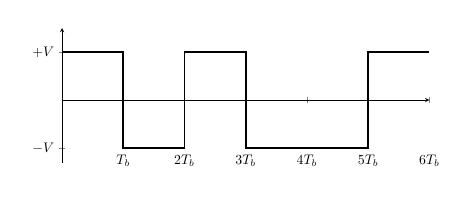
\begin{tikzpicture}[scale=0.5]
  \begin{axis}
    [axis lines = middle,width =0.9\linewidth,height=5cm,
    xmin= 0,xmax =6, ymin=-1.3,ymax=1.5,xtick={1,2,3,4,5,6},
    xticklabels={$T_b$,$2T_b$,$3T_b$,$4T_b$,$5T_b$,$6T_b$},
    xticklabel style={yshift = -1.2cm},
    ytick={-1,1},yticklabels={$-V$,$+V$}]
  \addplot[const plot, very thick] coordinates {(0,1) (1,-1) (2,1) (3,-1) (4,-1)
    (5,1) (6,1)};
\end{axis}
\end{tikzpicture}
  \caption{Codage NRZ binaire}
\end{figure}
\begin{defin}
  Pour un code NRZ binaire antipolaire on a:
  \[
    \begin{cases}
      a_k = + 1 & \text{ si } \beta_k =1 \\
      a_k = - 1 & \text{ si } \beta_k =0 \\
    \end{cases}
  \]
  Alors :
  \[
    m_a = 0 \text{ et } \sigma_a^2 = V^2
  \]
  Pour une forme d'impulsion rectangulaire on a donc:
  \[
    \phi_{ee}(f)= V^2 T_b \left(\frac{\sin\pi fT_b}{\pi f T_b}\right)^2+ \delta(f)\frac{V^2}{4}
  \]
\end{defin}

\subsubsection{Code NRZ binaire unipolaire}

\begin{figure}[H]
  \centering
  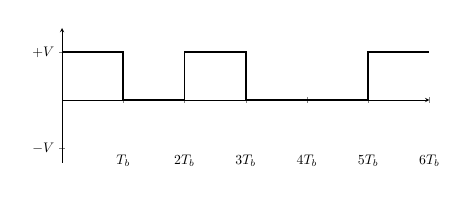
\begin{tikzpicture}[scale=0.5]
  \begin{axis}
    [axis lines = middle,width =0.9\linewidth,height=5cm,
    xmin= 0,xmax =6, ymin=-1.3,ymax=1.5,xtick={1,2,3,4,5,6},
    xticklabels={$T_b$,$2T_b$,$3T_b$,$4T_b$,$5T_b$,$6T_b$},
    xticklabel style={yshift = -1.2cm},
    ytick={-1,1},yticklabels={$-V$,$+V$}]
  \addplot[const plot, very thick] coordinates {(0,1) (1,0) (2,1) (3,0) (4,0)
    (5,1) (6,1)};
\end{axis}
\end{tikzpicture}
  \caption{Codage NRZ binaire}
\end{figure}
\begin{defin}
  Pour un code NRZ binaire unipolaire on a:
  \[
    \begin{cases}
      a_k = + 1 & \text{ si } \beta_k =1 \\
      a_k = 0 & \text{ si } \beta_k =0 \\
    \end{cases}
  \]
  Alors :
  \[
    m_a = +\frac{V}{2} \text{ et } \sigma_a^2 = \frac{V^2}{4}
  \]
  Pour une forme d'impulsion rectangulaire on a donc:
  \[
    \phi_{ee}(f)= \frac{V^2T_b}{4} \left(\frac{\sin\pi fT_b}{\pi f T_b}\right)^2
  \]
\end{defin}

\subsubsection{Code NRZ M-aire}
\begin{defin}
  On généralise le code NRZ binaire pour $a_k=\{\pm 1,\pm2 ... \pm
  (M/2-1)\}$ on a :
  \[  m_a = 0 \text{ et } \sigma_a^2 = \frac{2}{M} \sum_{p=0}^{(M/2)-1}(2p+1)^2
  \]
Pour une forme d'impulsion rectangulaire de durée $T=nT_b$on a donc:
  \[
    \phi_{ee}(f)= \frac{(M-1)^2}{3}V^3T \left(\frac{\sin\pi fT}{\pi f T}\right)^2
  \]
  
\end{defin}
\subsubsection{Code RZ binaire}

\begin{defin}
  On note $RZ_\lambda$ pour une impulsion rectangulaire de la forme:
  \[g(t)= 
    \begin{cases}
      +V & \forall t \in [0;\lambda T_b] \\
      0 & \forall t \in [\lambda T_b,T_b]
    \end{cases}
  \]
  Alors :
  \[
    \phi_{ee}(f)= \frac{V^2\lambda^2T_b}{4}\left(\frac{\sin\pi f_b\lambda T}{\pi f\lambda T_b}
    \right)^2 + \frac{V^2\lambda^2T_b}{4}\sum_{k=-\infty}^{+\infty} \left(\frac{\sin k\pi\lambda}{k\pi\lambda}\right)^2\delta(f-k/T_b)
  \]
\end{defin}
\begin{rem}
  Le plus classique est le code $RZ_{1/2}$:  on a une raie à $1/T_b$,
  mais pour une longue suite de $0$la DSP s'annule.
\end{rem}
\subsubsection{Code Manchester}
\begin{defin}
  \[
    \begin{cases}
      a_k = + 1 & \text{ si } \beta_k =1 \\
      a_k = 0 & \text{ si } \beta_k =0 \\
    \end{cases}
  \]
  Pour une impulsion rectangulaire on a donc:
  \[
      g(t)=
      \begin{cases}
        + V & \forall t \in [0,T_b/2] \\
        -V  & \forall t \in [T_b/2,T_b]\\
        0 & \forall t \notin [0,T_b]
      \end{cases}
    \]
    Alors:
    \[
 \phi_{ee}(f)= V^2T_b \left(\frac{\sin\pi fT_b/2}{\pi f T_b/2}\right)^2()\sin\pi fT_b/2)^2
    \]
\end{defin}

\begin{rem}
  Le codage de manchester est un transcodage ``1B2B'' : le 1 est
  codé par 1->0 alors que 0 est codé par 0->1. Les deux mots 11 et 00 ne
  sont pas utilisés. C'est le front montant ou descedant qui code l'information.

  La DSPd'un code de Manchester a une raie à la fréquence $f=1/T_b$,
  on peux faire de la synchronisation.
\end{rem}
\subsection{Code en Bande de base avec mémoire}
\subsubsection{Code bipolaire $RZ_{1/2}$}

\begin{defin}
  \[
    \begin{cases}
      a_k = \pm 1 & \text{ si } \beta_k =1 \\
      a_k = 0 & \text{ si } \beta_k =0 \\
    \end{cases}
  \]
 Donc $m_a =0$ et $\sigma_a^2 = 1/2$. 
  Pour une impulsion rectangulaire on a donc:
  \[
    g(t)=
    \begin{cases}
        + V & \forall t \in [0,T_b/2] \\
        -V  & \forall t \in [T_b/2,T_b]\\
    \end{cases}
  \]
  Alors :
  \[
    \phi_{ee}(f)= \frac{V^2T_b}{\sin^2(\pi fT_b)}\sinc^2(\frac{\pi fT_b}{2})
  \]
\end{defin}
\begin{prop}[Cas d'un code avec mémoire]
  Pour un code avec mémoire :
  \[
    \phi_{aa}(f) = \frac{\sigma_a^2}{T}+\frac{2\sigma_a^2}{T}\sum_{k=1}^{\infty}R_{aa}(k)\cos(2\pi fk T)+\frac{m_a^2}{T^2}\sum_{k=-\infty}^{+\infty}\delta(f-k/T)
  \]
  Avec $R_{aa}$ la fonction d'autocorrélation normalise des symboles
  $a_k$
  \[
    R_{aa}  = \frac{E[(a_n-m_a)(a_{n-k}-m_a)]}{\sigma_a^2}
  \]
\end{prop}

\begin{rem}
  $e(t)$ prend 3 niveaux de tension (+V,-V,0), ou 1 est codé
  alternativement par +V et -V. C'est un code
  \emph{pseudo-ternaire}. Si $\beta_k$ possède une longue suite de zéro la
  DSP va s'annuler...
\end{rem}

\subsubsection{Code HDBn}
\begin{defin}
  Pour éviter que la DSP s'annule on intercale des \emph{ bit de
    viols}pour limiter la succession de $n$ zéros.
\end{defin}
\begin{prop}
  Le $n$ de HBDn indique le nombre de 0 que l'on peut envoyer. On le choisit en fonction de la fiabilité du support et du matériel. La valeur pour le premier 1 à envoyer est fixée par convention entre l'émetteur et le récepteur.
\end{prop}


  \begin{center}
    \begin{tikzpicture}[
level distance=2cm,
level 1/.style={sibling distance=7cm},
level 2/.style={sibling distance=4.5cm},
      edge from parent fork down]
      \tikzset{if/.style={diamond,draw,aspect=2.5,inner sep=-3pt, label={[yshift=0.125cm]left:{\tiny\bf+}},
        label={[yshift=0.125cm]right:{\tiny-}},}}
      \node[if](I) {\begin{tabular}{c}
               Polarité du \\dernier viol
             \end{tabular}}
      [edge from parent path={[-latex] (\tikzparentnode) -| (\tikzchildnode)}]
  
      child {node[if] {
          \begin{tabular}{c}
            Polarité du \\dernier 1
          \end{tabular}}
        child {node {\texttt{-V00V}}}
        child {node {\texttt{000-V}}}
      }
      child {node[if] {
          \begin{tabular}{c}
            Polarité du \\dernier 1
          \end{tabular}}
        child {node {\texttt{000+V}}}
        child {node {\texttt{+V000+V}}}
      }
      ;
      \node[above=1cm] at (I.north) (O) {\texttt{0000}};
      \draw[-latex] (O) -- (I.north);
  \end{tikzpicture}
\end{center}


Pour compenser les bits de viols , on ajoute les \emph{ bits de bourrage.}
\begin{exemple}~\\
  \begin{figure}[H]
    \centering
  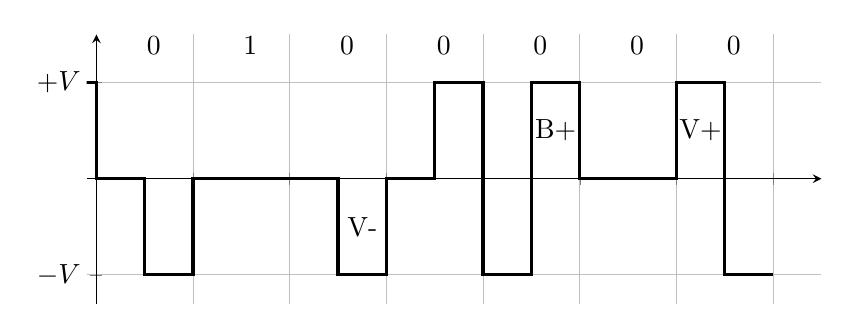
\begin{tikzpicture}
    \begin{axis}
    [axis lines = middle,width =0.9\linewidth,height=5cm,
    xmin= -0.2,xmax =15, ymin=-1.3,ymax=1.5,
    xticklabels={0,1,0,1,0,0,0,0,0,1,1,0,0,0,0,1},
    grid = major,
    xticklabel style={yshift = 2cm,xshift=-0.5cm},
    ytick={-1,1},yticklabels={$-V$,$+V$}]
    \addplot[const plot, very thick] coordinates {(-1,1) (0,0) (1,-1) (2,0)(3,0)(4,0)(5,-1)(6,0)(7,1)(8,-1)(9,1)(10,0)(11,0)(12,1)(13,-1)(14,-1)};  \node at (axis cs:5.5,-0.5){V-};
    \node at (axis cs:9.5,+0.5){B+};
    \node at (axis cs:12.5,+0.5){V+};
    \end{axis}
  \end{tikzpicture}
  \caption{Codage HDB3}
\end{figure}
\end{exemple}

\end{document}

%%% Local Variables:
%%% mode: latex
%%% TeX-master: t
%%% End:
